% This is samplepaper.tex, a sample chapter demonstrating the
% LLNCS macro package for Springer Computer Science proceedings;
% Version 2.20 of 2017/10/04
%
\documentclass[runningheads]{llncs}
%
\usepackage{graphicx}
\usepackage{latexsym}
\usepackage{amsmath}
\usepackage{float}
\usepackage{xspace}
\usepackage{algorithm}
\usepackage{algorithmic}
\usepackage{algorithmwh}
\usepackage{amssymb}
\usepackage{subfigure}
\usepackage{url}
\usepackage[mathscr]{eucal}
\usepackage{multirow}

% Used for displaying a sample figure. If possible, figure files should
% be included in EPS format.
%
% If you use the hyperref package, please uncomment the following line
% to display URLs in blue roman font according to Springer's eBook style:
% \renewcommand\UrlFont{\color{blue}\rmfamily}


\renewcommand{\algorithmicrequire}{\textbf{Input:}}
\renewcommand{\algorithmicensure}{\textbf{Output:}}

\newboolean{showcomments}
%
\setboolean{showcomments}{true}
\ifthenelse{\boolean{showcomments}}
{\newcommand{\nb}[2]{
\fbox{\bfseries\sffamily\scriptsize#1}
{\sf\small$\blacktriangleright$\textit{#2}$\blacktriangleleft$}
}
}
{\newcommand{\nb}[2]{}
}
\newcommand\amin[1]{\nb{Amin}{#1}}
\newcommand\ebrahim[1]{\nb{Ebrahim}{#1}}

\usepackage{mathtools}
%\DeclareMathOperator*{\argmax}{argmax}
\DeclareMathOperator*{\argmin}{argmin}
\DeclarePairedDelimiter{\norm}{\lVert}{\rVert}

\newcommand{\head}[1]{\par\smallskip\noindent\textbf{#1}}


\begin{document}
%
%\title{Link Prediction in Dynamic Heterogeneous Information Networks}
\title{Relationship Prediction in Dynamic Heterogeneous Information Networks}
%
%\titlerunning{Abbreviated paper title}
% If the paper title is too long for the running head, you can set
% an abbreviated paper title here
%

%\author{Amin Milani Fard\inst{1} \and Ebrahim Bagheri\inst{2} \and Ke Wang\inst{3}}

%\authorrunning{A. Milani Fard, E. Bagheri, K. Wang}
% First names are abbreviated in the running head. If there are more than two authors, 'et al.' is used.

%\institute{New York Institute of Technology, Vancouver, Canada\\ \email{amilanif@nyit.edu}\and Ryerson University, Toronto, Canada \\ \email{bagheri@ee.ryerson.ca}\\ \and
%Simon Fraser University, Burnaby, Canada\\ \email{wangk@cs.sfu.ca}}


\maketitle              % typeset the header of the contribution
%
\begin{abstract}

Most real-world information networks, such as social networks, are heterogeneous and as such, relationships in these networks can be of different types and hence carry differing semantics.
 %relations between different entities have different semantic meanings. 
 Therefore techniques for link prediction in homogeneous networks cannot be directly applied on heterogeneous ones. On the other hand, works that investigate link prediction in heterogeneous networks do not necessarily consider network dynamism in sequential time intervals. In this work we propose a technique that leverages a combination of latent and topological features to predict a target relationship between two nodes in a dynamic heterogeneous information network. Our technique, called MetaDynaMix, effectively combines meta path-based topology features and inferred latent features that incorporate temporal network changes in order to capture network (1) heterogeneity and (2) temporal evolution, when making link predictions. Our experiment results on two real-world datasets show statistically significant improvement over  AUCROC and prediction accuracy compared to the state of the art techniques.
%Our experiment results on two real-world datasets show 10-40\% increase in AUCROC, and 25-30\% increase in prediction accuracy compared to the state of the art techniques.
 
%\keywords{Link prediction \and Relationship prediction \and Dynamic heterogeneous networks \and Social networks \and Network topology \and Meta path.}

\end{abstract}
%\begin{abstract}
%The abstract should briefly summarize the contents of the paper in
%150--250 words.
%\keywords{First keyword  \and Second keyword \and Another keyword.}
%\end{abstract}
%
%
%

\section{Introduction}
\label{Sec:Introduction}

% what is link prediction problem? what is the usages of link prediction?

The goal of link prediction in a social network graph \cite{liben2007link} is to estimate the likelihood of the relationship between two nodes in future, based on the observed network. Predicting such connections in a network have multiple applications such as friend/item/ad recommending, network completion, or biological applications such as predicting protein-protein interactions.\amin{more citations} 

% challenges in heterogeneous link prediction, what is not covered? temporal and hero?

Traditional link prediction techniques \cite{liben2007link}\amin{more citations} consider social networks to be homogeneous, i.e., graphs with only one type of edges and nodes. However, most real-world social networks, such as Twitter, Facebook, and DBLP, are heterogeneous, i.e., they have multiple relation and node types. For example, in a bibliographic network there are different types of nodes such as authors, papers, and venues, and different types of edges such as write, cite and publish. There are limited number of works that focused on this problem. For example, the probabilistic latent tensor factorization model... Recent works, such as \cite{sun2011pathsim}, investigated this problem. However, such techniques do not consider the dynamics of social networks and ignore sequence of network snapshots. 
\amin{make sure about these citations}
\cite{Zhu2016} \cite{sun2011pathsim} \cite{Sun:2012:HRP:2124295.2124373}  \cite{huang2016meta} \cite{wang2016relsim} \cite{sun2013pathselclus} \cite{sun2011ASONAM} \cite{Yang2012} \cite{liben2007link}


In this work we study the problem of temporal and heterogeneous relashionship prediction that is stated as follows: \textit{Given a dynamic heterogeneous information network graph G (i.e., G has different types of nodes and links, attached with timestamps), how can we predict the future graph structure?}



\subsection{Motivation}

\amin{Motivate the problem by a real example and show the points made in this para.}

The link prediction problem for homogeneous networks has been studied in the past \cite{liben2007link}\amin{more citations}. However most real social networks are heterogeneous and relations between different entities have different semantic meanings. Thus techniques for homogeneous networks can not be directly applied on heterogeneous ones. A few works, such as \cite{sun2011pathsim,sun2011ASONAM}, investigated this problem, however, they do not consider the dynamics of social networks and ignore ignore sequence of network snapshots. On the other hand, it has ben shown that for homogenous network link prediction, incorporating temporal changes helps in a more accurate prediction \cite{Zhu2016}. Previous work on temporal link prediction scarcely studied heterogeneousness of social networks and to the best of our knowledge, the problem of relationship prediction for dynamic heterogeneous networks was not studied before.


\subsection{Contributions}

The main contributions of our work include:

\begin{itemize}

\item We present a technique, called \texttt{RelationPredict}, that predicts a target relationships between two nodes of given types;

\item An evaluation of the accuracy and performance of the proposed algorithm on real social network data.

\end{itemize}



\section{Problem Statement}


Our work is focused on heterogeneous information networks (graphs) that can change and evolve over time. As such, we first formally define the concept of \textit{Dynamic Heterogeneous Information Networks}, as follows:

%In this section, we briefly introduce some concepts related to heterogeneous information network and the relationship prediction problem. A HIN is a directed graph that may contain multiple types of nodes and links. The following definition is an extended version of HIN \cite{sun2011pathsim} that we use to formally define a dynamic HIN.

\begin{definition}[\textbf{Dynamic heterogeneous information network}] A dynamic heterogeneous information network (DHIN) is a directed graph $G$ = ($V$, $E$) with a node type mapping function $\phi: V \rightarrow \mathcal{A}$ and a link type mapping function $\psi: E \rightarrow \mathcal{R}$, where $V$, $E$, $\mathcal{A}$, and $\mathcal{R}$ denote sets of nodes, links, node types, and relation types, respectively. Each node $v \in V$ belongs to a node type $\phi(v)\in \mathcal{A}$, each link $e\in E$ belongs to a relation $\psi(e)\in \mathcal{R}$, and $|\mathcal{A}| > 1$ and $|\mathcal{R}| > 1$. Also each edge $e = (u, v, t)$ connects two vertices $u$ and $v$ with a timestamp $t$.$\Box$ \end{definition}%is a temporal edge from $u$ to $v$ at time $t$. $\Box$ \end{definition}



The DBLP bibliographic network %\footnote{\url{http://dblp.uni-trier.de/db/}} 
is an example of a DHIN, containing different types of nodes such as papers, authors, topics, and publication venues, with publication links associated with a date. %Another example is the Twitter social network with nodes types such as tweets, users, topics, and hashtags, and a timestamp associated with these tweets. 
In the context of a heterogenous network, a \textit{relation} can be in the form of a \textit{direct link} or an \textit{indirect link}, where an indirect link is a sequence of direct links in the network. Thus, two nodes might not be directly connected, however they might be considered to be indirectly connected through a set of intermediary links. In this work, we use the terms \textit{relationship prediction} and \textit{link prediction} interchangeably referring to predicting whether two nodes will be connected in the future via a \textit{sequence of relations} in the graph, where the \textit{length} of a sequence is greater than or equal to one. For instance in a bibliographic network, a direct link exists between an author and a paper she wrote, and an indirect link exists between her and her co-authors through the paper, which they wrote together. In order to better capture different types of nodes and their relation in a network, the concept of \textit{network schema} \cite{sun2011pathsim} is used. A network schema is a meta graph structure that summarizes a HIN and is formally defined as follows:

\begin{definition}[\textbf{Network schema}]For a heterogeneous network $G=(V,E)$, the network schema $S_G=\mathcal{(A,R)}$ is a directed meta graph where $\mathcal{A}$ is the set of node types in $V$ and $\mathcal{R}$ is the set of relation types in $E$.  $\Box$\end{definition}

Figure \ref{schema} shows the network schema for the DBLP bibliographic network with $\mathcal{A}$=\{\textit{Author}, \textit{Paper}, \textit{Venue}, \textit{Topic}\}. In this paper, we refer to different types of nodes in the DBLP bibliographic network with abbreviations $P$ for paper, $A$ for author, $T$ for topic, and $V$ for venue. 

\begin{figure}[t]
\centering
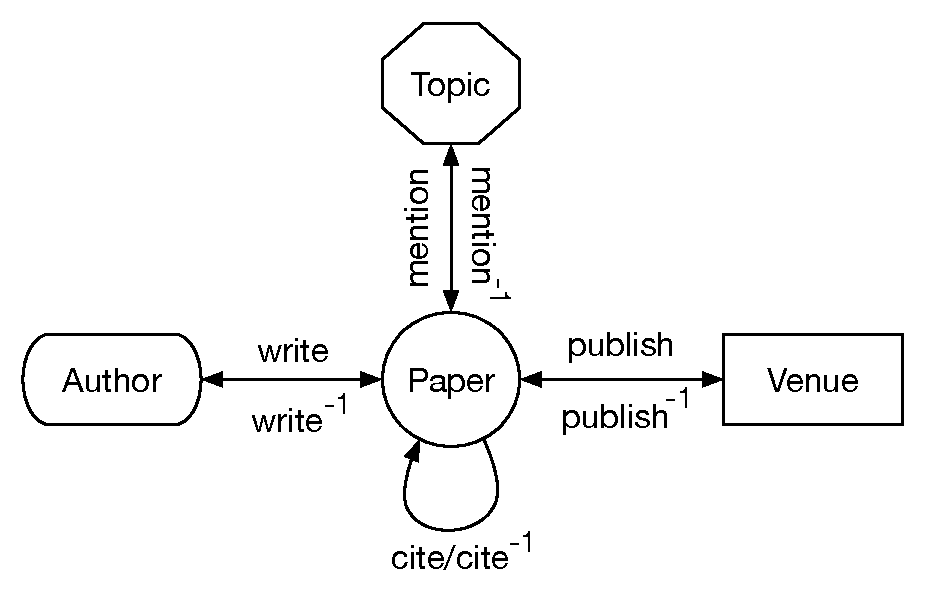
\includegraphics[trim = 0mm 10mm 0mm 5mm,width=0.46\textwidth]{figs/schema.pdf}
\caption{Network schema for DBLP network.}\label{schema}
\end{figure}

%\subsection{Meta path-based topology}

Similar to the notion of network schema that provides a meta structure for the network, a \textit{meta path} \cite{sun2011pathsim} provides a meta structure for paths between different node types in the network. 

\begin{definition}[\textbf{Meta path}]A meta path $\mathcal{P}$ is a path in a network schema graph $S_G = (\mathcal{A,R})$, denoted by $\mathcal{P}(A_1,A_{n+1}) = A_1 \xrightarrow{R_1} A_2... \xrightarrow{R_n} A_{n+1}$, as a sequence of links between node types defining a composite relationship between a node of type $A_1$ and one of type $A_{n+1}$, where $A_i \in \mathcal{A}$ and $R_i \in \mathcal{R}$. $\Box$\end{definition}

The \textit{length} of a meta path is the number of relations in it. Note that given two node types $A_i$ and $A_j$, there may exist multiple meta paths of different lengths between them. We call a path $p = (a_1a_2...a_{n+1})$ a \textit{path instance} of a meta path $\mathcal{P} = A_1-A_2... -A_{n+1}$ if $p$ follows $\mathcal{P}$ in the corresponding HIN, i.e., for each node $a_i$ in $p$, we have $\phi(a_i)=A_i$. The co-author relationship in DBLP can be described with the meta path $A\xrightarrow{write}P\xrightarrow{write^{-1}}A$ or in short \textit{A--P--A}. Paths in thick solid lines in Figure \ref{sampleNetwork} correspond to \textit{A--P--V--P--A} meta paths between \textit{Max} and \textit{Ada}, indicating they published in the same venue, such as \textit{Max--P1--ECIR--P3--Ada}. Each meta path carries different semantics and defines a unique topology representing a special relation. %The relationship between two authors are different in meaning when they are co-authors (\textit{A--P--A}) versus one citing another's paper (\textit{A--P--P--A}).

\begin{figure}[t]
\centering
%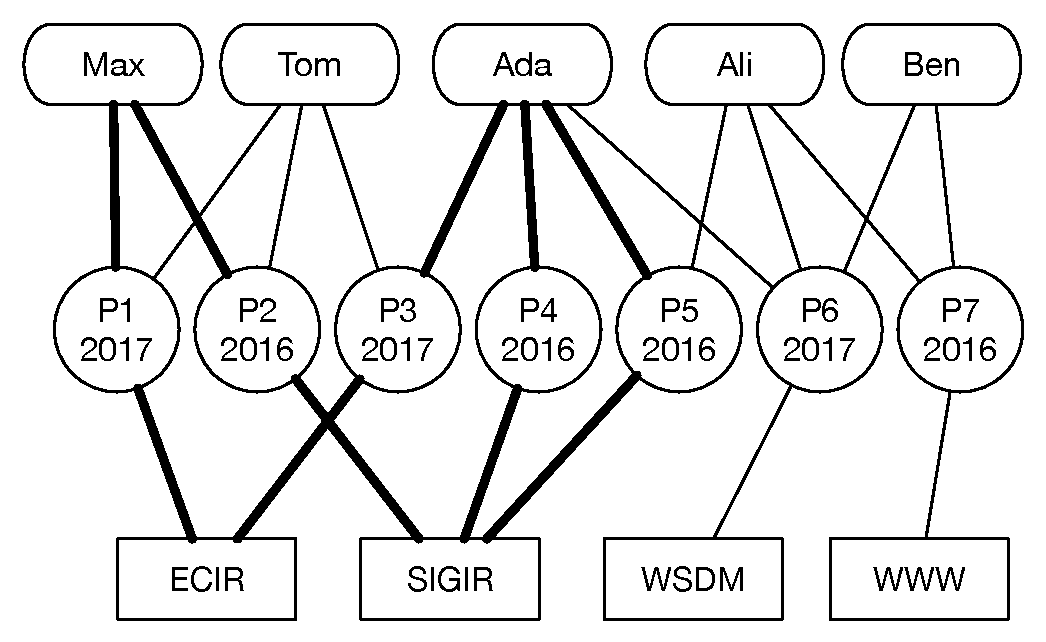
\includegraphics[width=0.42\textwidth]{figs/exampleSocialNetwork.pdf}
\subfigure[An example of \textit{A--P--V--P--A} meta paths between two authors Max and Ada.]{
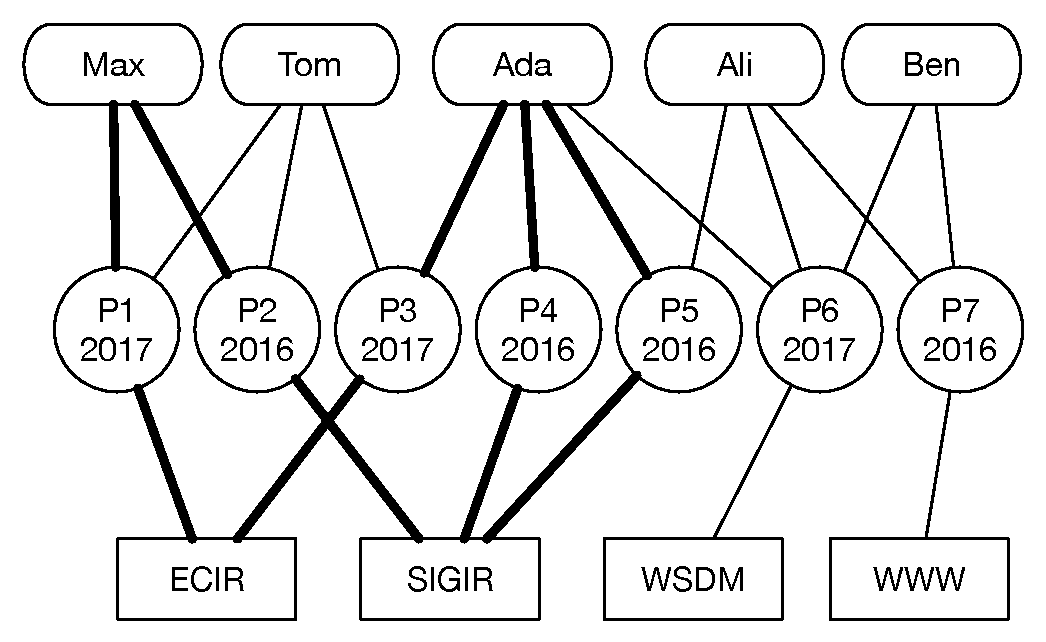
\includegraphics[trim = 0mm -5mm 0mm 5mm,width=0.52\hsize]{figs/exampleSocialNetwork.pdf}
 \label{sampleNetwork}
}\hspace{0.6cm}
\subfigure[The augmented reduced graph based on $\mathcal{P}(A,A)$=\textit{A--P--V--P--A}]{
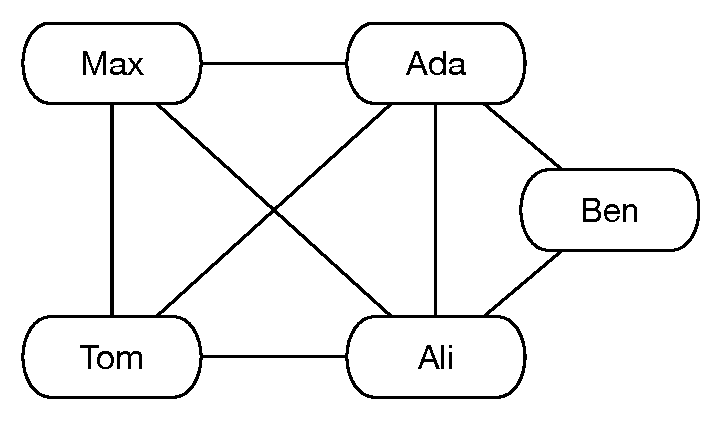
\includegraphics[trim = 0mm -20mm 0mm 5mm,width=0.38\hsize]{figs/exampleARG.pdf}
 \label{arg}
}\vspace{-2mm}
\caption{An example of a publications network. Link formation time is shown below the paper ID.}
%\label{sampleNetwork}
\end{figure}


\textbf{Meta Path-based Similarity Measures.} Given a meta path $\mathcal{P} = (A_i,A_j)$ and a pair of nodes $a$ and $b$ such that $\phi(a)=A_i$ and $\phi(b)=A_{j}$, several \textit{similarity measures} can be defined between $a$ and $b$ based on the path instances of $\mathcal{P}$. Examples of such similarity or proximity measures in a HIN are \textit{path count} \cite{sun2011pathsim,sun2011ASONAM}, \textit{PathSim} \cite{sun2011pathsim} or \textit{normalized path count} \cite{sun2011ASONAM}, \textit{random walk} \cite{sun2011ASONAM}, \textit{HeteSim} \cite{shi2014hetesim}, and \textit{KnowSim} \cite{wang2016text}. 
%Given a meta path $\mathcal{P}$ a source node $a$ and a target node $b$, path count measures the number of path instances between $a$ and $b$ following $\mathcal{P}$, and can be calculated by multiplying adjacency matrices of relations in $\mathcal{P}$ \cite{sun2011ASONAM}, and random walk is the probability of the random walk that starts from $a$ and ends with $b$ following $\mathcal{P}$. 
%More discussion about these similarity measures can be found in \cite{shi2014hetesim,sun2011ASONAM,sun2011pathsim,wang2016text}. 
Without loss of generality, in this work, we use Path Count (PC) as the default similarity measure. For example, given the meta path \textit{A--P--V--P--A} and the HIN in Figure \ref{sampleNetwork}, $PC(Max,Ada)$=3 and $PC(Tom,Ada)$=4. We now formally define the problem that we target in this work as follows:

\begin{definition}[\textbf{Relationship prediction problem}]\label{problemdef}Given a DHIN graph $G$ at time $t$, and a target relation meta path $\mathcal{P}(A_i,A_j)$ between nodes of type $A_i$ and $A_j$, we aim to predict the existence of a path instance of $\mathcal{P}$ between two given nodes of types $A_i$ and $A_j$ at time $t+1$. $\Box$ \end{definition}


%Tom-P3-ECIR-P3-Ada
%Tom-P1-ECIR-P3-Ada
%Tom-P2-SIGIR-P4-Ada
%Tom-P2-SIGIR-P5-Ada
%
%Max-P1-ECIR-P3-Ada
%Max-P2-SIGIR-P4-Ada
%Max-P2-SIGIR-P5-Ada


% Removed for ECIR version

%In the Table \ref{table_notations} summarizes the notations frequently used throughout the paper. 
%
%\begin{table}[t]
%\centering
%\caption{Notations and their description.}
%\label{table_notations}
%\begin{tabular}{|c|l|} 
%
%\hline\textbf{Notation} & \textbf{Description} \\ \hline
%$\mathcal{A}$, $\mathcal{R}$  & Types of nodes and relations \\ \hline
%$\phi$, $\psi$  & Mapping functions for node type and link type  \\ \hline
%$\mathcal{P}$, $p$  & A Meta path and a path instance \\ \hline
%$f^{\mathcal{P}}(x,y)$ & Meta path-based feature measures based on $\mathcal{P}$ \\ \hline
%$G_\tau$, $\hat{G}_\tau$ & Graph $G$ and predicted $G$ at time $\tau$  \\ \hline
%$G^\mathcal{P}$ & Augmented reduced graph based on $\mathcal{P}$ \\ \hline
%$Z_\tau$ & Latent space representation matrix for $G_\tau$ \\ \hline
%$k$ & The dimension of latent features \\ \hline
%
%\end{tabular}
%\end{table}





%By checking the existing topological features defined in homogeneous networks, we can find that both the neighbor set-based features and path-based features can be generalized in heterogeneous information networks, by considering paths following different meta paths. For example, if we treat each type of neighbors separately and extend the immediate neighbors to n-hop neighbors (i.e., the distance between one object and its neighbors are n), the common neighbor feature between two authors is then becoming the count of paths between the two authors following different meta paths. For path-based features, such as Katz, it can be extended as a combination of paths following different meta paths. 
\section{Proposed Relationship Prediction Approach}

Given a DHIN graph $G=(V,E)$, we first decompose $G$ to a sequence of $t$ HIN graphs ${G_1, .., G_t}$ based on links with associated timestamps. We then apply our techniques to predict relationships in $G_{t+1}$. As mentioned in Definition \ref{problemdef}, we intend to predict existence of a given type of relationship (target meta path) between two given nodes. Thus we define a new type of graph, called \textit{augmented reduced graph}, that is generated according to a given heterogeneous network and a target relation meta path. 

%\begin{definition}[Augmented reduced graph]\label{def:ARG}
%Given a HIN graph $G=(V,E)$ and a target meta path $\mathcal{P}(A_i,A_j)$ between nodes of type $A_i$ and $A_j$, an \textit{augmented reduced graph} $G^\mathcal{P}=(V^\mathcal{P},E^\mathcal{P})$ is a weighted graph, where $V^\mathcal{P} \subseteq V$ and nodes in $V^\mathcal{P}$ are of type $A_i$ and $A_j$, edges in $E^\mathcal{P}$ indicates relationships of type $\mathcal{P}$ in $G$, and each edge $e^\mathcal{P} = (u, v, w)$ is a weighted edge from a vertex $u$ to a vertex $v$ with a weight $w=Sim(u,v)$ indicating a similarity measure between $u$ and $v$. $\Box$
%\end{definition}

\begin{definition}[\textbf{Augmented reduced graph}]\label{def:ARG}
Given a HIN graph $G=(V,E)$ and a target meta path $\mathcal{P}(A_i,A_j)$ between nodes of type $A_i$ and $A_j$, an \textit{augmented reduced graph} $G^\mathcal{P}=(V^\mathcal{P},E^\mathcal{P})$ is a graph, where $V^\mathcal{P} \subseteq V$ and nodes in $V^\mathcal{P}$ are of type $A_i$ and $A_j$, and edges in $E^\mathcal{P}$ indicates relationships of type $\mathcal{P}$ in $G$. $\Box$
\end{definition}


For example, an augmented reduced graph for the network in Figure \ref{sampleNetwork} and target meta path $\mathcal{P}(A,A)$=\textit{A--P--V--P--A} is a graph whose nodes are of type \textit{Author} and whose edges represent \textit{publishing in the same venue}. %For example (\textit{Max}, \textit{Ada}) is an edge in the corresponding augmented reduced graph because they both published at KDD and ICDM. If we consider meta path $\mathcal{P}(A,A)$=\textit{A--P--A}, the augmented reduced graph represents a co-authorship graph, where nodes are of type \textit{Author} and edges, such as (\textit{Max}, \textit{Tom}), represent \textit{co-authorship}.

%\subsection{Algorithm}

\subsection{Homogenized link prediction}

Once the given DHIN graph $G=(V,E)$ is decomposed to $t$ HIN graphs $G_1, .., G_t$, one solution to the relationship prediction problem (Definition \ref{problemdef}) is to build an augmented reduced graph $G_i^\mathcal{P}$ for each $G_i$ with respect to the given target meta path $\mathcal{P}$ and then predict a link in $G_i^\mathcal{P}$ instead of a path in $G_i$. In other word, we generate a homogenize the given graph and apply a link prediction method.

Zhu et al. \cite{Zhu2016} studied the problem of temporal link prediction in the context of homogeneous networks where the input is a sequence of graphs $G_1, ..., G_t$ and the output is the estimated $G_{t+1}$. They present a matrix factorization (MF) with block-coordinate gradient descent which infers a low rank $k$-dimensional latent space matrix $Z_\tau$ for each adjacency matrix $G_\tau$ at time $\tau$ by minimizing 
\begin{equation}\label{latentOrigEqu}
    \begin{array}{l}
\argmin\limits_{Z_1, .., Z_t}\sum\limits_{\tau=1}^{t}\left \| G_\tau-Z_{\tau}Z_{\tau}^T \right \|^2_F+\lambda \sum\limits_{\tau=1}^{t}\sum\limits_{u}(1-Z_{\tau}(u)Z_{\tau-1}(u)^T) 
\\
\text{subject to :} \forall u,\tau,Z_{\tau}\geq 0, Z_{\tau}(u)Z_{\tau}(u)^T=1
    \end{array}
\end{equation}
where $\lambda$ is a regularization parameter, and  $(1-Z_{\tau}(u)Z_{\tau-1}(u)^T)$ penalizes node $u$ for suddenly changing its latent position. %Note that when computing the quadratic loss $\left \| G^R_\tau-Z_{\tau}BZ_{\tau}^T \right \|^2_F$, we ignore all of the diagonal entries.
$Z_\tau(u)$ is a row vector denoting $u$'s temporal latent space representation at time $\tau$, and $Z_\tau(u,i)$ indicates the position of $u$ in the $i$-th dimension at $Z$. The intuition behind their technique is that 1) nodes move smoothly in the latent space over time and it is less likely to have abrupt moves \cite{sarkar2005dynamic,zhang2014inferring}, and 2) user interactions are more likely to occur between similar users in a latent space representation. To predict adjacency matrix $G_{t+1}$, they used $Z_tZ_t^T$, however, they mentioned that $G_{t+1}$ can be formulated as $\Phi(f(Z_1,...Z_t))$, where $\Phi$ and $f$ are link and temporal functions that one may apply techniques such as nonparametric approaches \cite{Sarkar:2012} to learn them.

Algorithm \ref{alg1} is an adaptation of the above MF technique applied on a sequence of augmented reduced graphs $G^\mathcal{P}_i$ (Definition \ref{def:ARG}) given a target meta path $\mathcal{P}$, which changes Equation (\ref{latentOrigEqu}) by replacing $G_\tau$ with $G^\mathcal{P}_\tau$.
%to the following
%\begin{equation}\label{latentReducedEqu}
%    \begin{array}{l}
%\argmin\limits_{Z_1, .., Z_t}\sum\limits_{\tau=1}^{t}\left \| G^\mathcal{P}_\tau-Z_{\tau}Z_{\tau}^T \right \|^2_F+\lambda \sum\limits_{\tau=1}^{t}\sum\limits_{u}(1-Z_{\tau}(u)Z_{\tau-1}(u)^T) 
%\\
%\text{subject to :} \forall u,\tau,Z_{\tau}\geq 0, Z_{\tau}(u)Z_{\tau}(u)^T=1
%    \end{array}
%\end{equation}
%Their MF technique \cite{Zhu2016} to infer $Z_t$ and estimate $G_{t+1}^R$. We refer to this approach as \texttt{HomoTemp}.
The algorithm gets as input a DHIN graph $G$, the number of graph snapshots $t$, a target relation meta path $\mathcal{P}(A,B)$, the latent space dimension $k$, and the link to predict $(a,b)$ at $t+1$. The algorithm first decomposes $G$ into a sequence of $t$ graphs $G_1, .., G_t$ by considering the associated timestamps on edges (line 1). Next from each graph $G_i$, a corresponding augmented reduced graph $G^\mathcal{P}_i$ is generated (lines 2-7) for which nodes are of type $a$ and $b$ (beginning and end of target  meta path $\mathcal{P}$). For example given $\mathcal{P}(A,A)$=\textit{A--P--A}, each $G^\mathcal{P}_i$ represents the co-authorship graph at time t. Finally the matrix factorization technique in \cite{Zhu2016} is applied (line 8) to infer latent spaces $Z_1, ...,Z_t$ and estimate $G^\mathcal{P}_{t+1}$ by $Z_tZ_t^T$ (line 9). Note that $Z_\tau$ depends on $Z_{\tau-1}$ as used in the temporal regularization term in Equation (\ref{latentOrigEqu}).



\begin{algorithm}[t]
\caption{Homogenized Link Prediction}\label{alg1}
\begin{algorithmic}[1]\scriptsize
\REQUIRE A DHIN graph $G$, the number of snapshots $t$, a target meta path $\mathcal{P}(A,B)$, the latent space dimension $k$, the link to predict $(a,b)$ at $t+1$
%\ENSURE The predicted graph $G^\mathcal{P}$ at time $t+1$ based on the target relation $\mathcal{P}$
\ENSURE The probability of existence of link $(a,b)$ in $G^\mathcal{P}_{t+1}$

\STATE $\{G_1, .., G_t\} \leftarrow DecomposeGraph(G, t)$

\FOR {each graph $G_i=(V_i,E_i)$}
    %\STATE $G^R_i \leftarrow AugmentedReducedGraph(G_i,P,S)$
    %\STATE Let $a$ and $b$ be the node types of beginning and end of $\mathcal{P}$
    
    %\FOR {each path $p$ between nodes of type $a$ and $b$ in $S$}
    \FOR {each node $x \in V_i$ that $\phi(x)=A$}%of type $a$}
        \STATE Follow $\mathcal{P}$ to reach a node $y\in V_i$ that $\phi(y)=B$%of type $b$ 
        \STATE Add nodes x and y, and edge $(x,y)$ to the augmented reduced graph $G_i^\mathcal{P}$ 
\ENDFOR

\ENDFOR
%\STATE $G^R_{t+1} \leftarrow MF(G^R,k)$ \cite{Zhu2016}
%\STATE Infer temporal latent spaces $Z_1, .., Z_t$ using \textit{MF}%by optimizing Eq. \ref{latentReducedEqu}
\STATE $\{Z_1, .., Z_t\} \leftarrow MatrixFactorization(G^\mathcal{P}_1, .., G^\mathcal{P}_t, k)$

\STATE Return $Pr((a,b)\in E^\mathcal{P}_{t+1}) \leftarrow \sum_{i=1}^{k} Z_t(a,i)Z_t(b,i)$


%\STATE $G^\mathcal{P}_{t+1} \leftarrow Z_tZ^T_t$ 
%\STATE Return $G^\mathcal{P}_{t+1}$
\end{algorithmic}
\end{algorithm}


%\subsection{Meta path-based relationship prediction}
\subsection{Dynamic meta path-based relationship prediction}

The above homogenized approach does not consider different semantics of meta paths between the source and destination nodes. In fact, Zhu et al. \cite{Zhu2016} assume that the probability of a link between nodes depends only on their latent positions. On the other hand, Sun et al. \cite{sun2011ASONAM} proposed a supervised learning framework, called \textit{PathPredict}, that uses meta path-based features in a past time interval to predict the relationship building in a future time interval. It learns coefficients associated with features by maximizing the likelihood of new relationship formation. However, their model is learned based on one past interval and does not consider temporal changes as in \cite{Zhu2016}. Our intuition is that leveraging meta path-based features along with latent space features can help to boost the prediction accuracy. In other word, we combine latent space features with topological meta path-based features in our predictive model.


\begin{algorithm}[t]
\caption{Dynamic Meta path-based Relationship Prediction}\label{alg2}
\begin{algorithmic}[1]\scriptsize
\REQUIRE A DHIN graph $G$, the number of snapshots $t$, a network schema $S$, a target meta path $\mathcal{P}(A,B)$, the maximum length of a meta path $l$, the latent space dimension $k$, the link to predict $(a,b)$ at $t+1$
%\ENSURE The predicted graph $G^\mathcal{P}$ at time $t+1$ based on the target relation $\mathcal{P}$
\ENSURE The probability of existence of link $(a,b)$ in $G^\mathcal{P}_{t+1}$

\STATE $\{G_1, .., G_t\} \leftarrow$ \textit{DecomposeGraph}$(G, t)$
%\STATE  $\{G^\mathcal{P}_1, .., G^\mathcal{P}_t\} \leftarrow BuildTargetAugmentedReducedGraph(G_1, .., G_t, \mathcal{P}(a,b))$
\STATE  Generate target augmented reduced graphs $G^\mathcal{P}_1, .., G^\mathcal{P}_t$ following Algorithm 1 lines 2-7

\STATE $\{\mathcal{P}_1, .., \mathcal{P}_n\} \leftarrow$ \textit{GenerateMetaPaths}$(S, \mathcal{P}(A,B), l)$

%\FOR {each graph $G_i=(V_i,E_i)$}
%
%    \FOR {each node $x \in V_i$ that $\phi(x)=A$}%of type $a$}
%	\FOR {each meta path $\mathcal{P}_j$}
%
%        \STATE Follow $\mathcal{P}_j$ to reach a node $y$ that $\phi(y)=B$%of type $b$}
%        \STATE $w_{xy} \leftarrow Similarity(x,y, G_i)$
%        \STATE Add nodes x and y, and edge $(x,y)$ with weight $w_{xy}$ to augmented reduced graph $G_i^{\mathcal{P}_j}$ 
%\ENDFOR
%\ENDFOR

%\STATE $\{Z_1, .., Z_t\} \leftarrow MatrixFactorization(G^{\mathcal{P}_j}_1, .., G^{\mathcal{P}_j}_t, k)$
%\STATE $G^{\mathcal{P}_j}_{t+1} \leftarrow Z_tZ^T_t$ 

%\ENDFOR

\STATE $\{Z_1, .., Z_t\} \leftarrow$ \textit{MatrixFactorization}$(G^\mathcal{P}_1, .., G^\mathcal{P}_t, k)$
\STATE $\hat{G}^\mathcal{P}_{t} \leftarrow Z_{t-1}Z^T_{t-1}$ and  $\hat{G}^\mathcal{P}_{t+1} \leftarrow Z_tZ^T_t$


\FOR {each pair $(x,y)$, where $x\in V^\mathcal{P}_{t-1}$ and $y\in N(x)$ is a nearby neighbor of $x$ in $G^\mathcal{P}_{t-1}$}

\STATE Add the feature vector $\langle$ $f^{\mathcal{P}_1}_{t-1}(x,y)$, $f^{\mathcal{P}_2}_{t-1}(x,y)$, ..., $f^{\mathcal{P}_n}_{t-1}(x,y)$, $\hat{G}^\mathcal{P}_{t}(x,y)\rangle$ to the training set $T$ with \textit{label}=1 if $(x,y)$ is a new link in $E^\mathcal{P}_{t}$ otherwise \textit{label}=0.

\ENDFOR

%\STATE $\forall (a,b\in N(a)) \in G^\mathcal{P}_{t}$, add a feature vector to the training set with $w_{ab}$ in $G^{\mathcal{P}_j}_{t-1}$ for each meta paths $\mathcal{P}_j$, and label=1 if $(a,b) \in E^\mathcal{P}_{t}$ otherwise label=0.

%\STATE Learn the model and apply it to the feature vector of $G^{\mathcal{P}_j}_{t+1}$ with different meta path $\mathcal{P}_j$.

\STATE $model \leftarrow$ \textit{Train}$(T)$
\STATE Return $Pr((a,b)\in E^\mathcal{P}_{t+1})$ $\leftarrow$ \textit{Test}($model$, $\langle$ $f^{\mathcal{P}_1}_{t}(a,b)$, $f^{\mathcal{P}_2}_{t}(a,b)$, ..., $f^{\mathcal{P}_n}_{t}(a,b)$, $\hat{G}^\mathcal{P}_{t+1}(a,b)\rangle)$

%\STATE Build $G^\mathcal{P}_{t+1}$ based on the cut-off values for the output of prediction model.
%\STATE Return $G^\mathcal{P}_{t+1}$
\end{algorithmic}
\end{algorithm}

Algorithm \ref{alg2} gets as input a DHIN graph $G$, the number of graph snapshots $t$, a network schema $S$, a target relation meta path $\mathcal{P}(A,B)$, the maximum length of a meta path $l$, the latent space dimension $k$, and the link to predict $(a,b)$ at $t+1$. Same as Algorithm \ref{alg1}, it decomposes $G$ into a sequence of graphs (line 1). Next it generates augmented reduced graphs $G^\mathcal{P}_i$s from $G_i$s based on $\mathcal{P}$ for which nodes are of type $A$ and $B$ (beginning and end of meta path $\mathcal{P}$) (line 2) as explained in Algorithm 1. It then produces the set of all meta paths between nodes of type $A$ and type $B$ defined in $\mathcal{P}(A,B)$ (line 3). This is done by traversing the network schema $S$ (for instance through a BFS traversal) and generating meta paths with the maximum length of $l$. It then applies the MF technique \cite{Zhu2016} to find latent space matrices $Z_i$ (line 4).On this basis, it then calculates the estimated augmented reduced graph $\hat{G}^\mathcal{P}$ at times $t$ and $t+1$ (line 5). The last steps create a training dataset with sample pairs $(x,y)$ with feature set containing $\hat{G}^\mathcal{P}_{t}(x,y)$, and meta path-based feature measures $f^{\mathcal{P}_i}_t(x,y)$ based on meta path $\mathcal{P}_i$ at time $t$, and \textit{label}=1 if $(x,y)$ is a new link in $G^\mathcal{P}_{t+1}$ otherwise \textit{label}=0 (lines 6-8), subsequently training the predictive model (line 9), generating features for the given pair $(a,b)$ and testing it using the trained model (line 10). In the following section we explain our learning technique in detail.

% \begin{equation}\label{latentEqu}
%     \begin{array}{l}
% \argmin\limits_{Z_1, .., Z_t}\sum\limits_{\tau=1}^{t}\left \| G^{R_i}_\tau-Z_{\tau}Z_{\tau}^T \right \|^2_F+\lambda \sum\limits_{\tau=1}^{t}\sum\limits_{u}(1-Z_{\tau}(u)Z_{\tau-1}(u)^T) 
% \\
% \text{subject to :} \forall u,\tau,Z_{\tau}\geq 0, Z_{\tau}(u)Z_{\tau}(u)^T=1
%     \end{array}
% \end{equation}


%* Restrict pathSim to 3-hops and not beyond


%\begin{equation}\label{latentAndTopologicalEqu}
%    \begin{array}{l}
%\argmin\limits_{\boldsymbol{\theta},Z_1, .., Z_t}\sum\limits_{\tau=1}^{t}\left \| G_\tau - (Z_{\tau}Z_{\tau}^T + \sum\limits_{i=1}^{n}\theta_{i_\tau}\mathcal{F}_{i_\tau}) \right \|^2_F + \lambda (\sum\limits_{\tau=1}^{t}\sum\limits_{u}(1-Z_{\tau}(u)Z_{\tau-1}(u)^T)  + \sum\limits_{\tau=1}^{t} \sum\limits_{i=1}^{n} \theta_{i_\tau}^2)\\
%    \end{array}
%\end{equation}


%\subsubsection{The predictive model.}
\subsubsection{Combining latent and meta path-based features.}
Our hypothesis is that combining latent with topological features can increase the prediction accuracy as we can learn latent features that fit the residual of meta path-based features. However, if the latent features learn similar structure to the topological features, then mixing them may not be beneficial. One way to do so is by changing the loss function in Equation (\ref{latentOrigEqu}) to $\argmin\limits_{\boldsymbol{\theta_\tau},Z_\tau}\sum\limits_{\tau=1}^{t}\left \| G^\mathcal{P}_\tau - \Phi(Z_{\tau}Z_{\tau}^T + \sum\limits_{i=1}^{n}\theta_{i_{\tau-1}} \mathcal{F}^{\mathcal{P}_i}_{\tau-1}) \right \|^2_F$ and adding another regularization term $\lambda \sum\limits_{\tau=1}^{t} \sum\limits_{i=1}^{n} \theta_{i_\tau}^2$, where $n$ is the number of meta path-based features, $\mathcal{F}^{\mathcal{P}_i}$ is the $i$-th meta path-based feature matrix defined on $G_i$, and $\theta_i$ is the weight for feature $f_i$. Although the gradient descent algorithm used in the MF technique to infer latent space matrices in \cite{Zhu2016} is fast, it cannot be efficiently applied to the changed loss function. This is because it requires computing meta paths for all possible pairs of nodes in $\mathcal{F}^{\mathcal{P}_i}$ for all snapshots, which is not scalable as calculating similarity measures such as PathCount or PathSim can be very costly. For example computing path counts for \textit{A--P--V--P--A} meta path, can be done by multiply adjacency matrices $AP\times PV\times VP\times PA$. 


%Thus we restrict it only to those links that make new connections in the next time interval or negative samples and use logistic regression.
As an alternative solution, we build a predictive model that considers a linear combination of topological and latent features. These features, however, can be combined in different ways that is beyond the scope of this work. Given the training pairs of nodes and their corresponding meta path-based and latent features, we apply logistic regression to learn the weights associated with these features. We define the probability of forming a \textit{new link} in future from node $a$ to $b$ as %$Pr(label=1|a, b; \boldsymbol{\theta}) = \frac{1}{e^{-z}+1}$, where $z=\sum\limits_{i=1}^{n}\theta_i.f_i(a,b)$ 
 $Pr(label=1|a, b; \boldsymbol{\theta}) = \frac{1}{e^{-z}+1}$, where $z=\sum\limits_{i=1}^{n}\theta_i f^{\mathcal{P}_i}(a,b) + \sum\limits_{j=1}^{k} \theta_{n+j}Z(a,j)Z(b,j)$, and $\theta_1,\theta_2,..., \theta_n$ and $\theta_{n+1},\theta_{n+2},..., \theta_{n+k}$ are associated weights for meta path-based features and latent features at current time between $a$ and $b$. Given a training dataset with $l$ instance-label pairs, we use logistic regression with $L_2$ regularization to estimate the optimal $\boldsymbol{\theta}$ as%where $\lambda \sum_{j=1}^{n+k} \theta_j^2$ is the regularization term, and $C>0$ is a penalty parameter. 

%$\boldsymbol{\hat{\theta}} = 
%\operatorname*{arg\,max}_{\boldsymbol{\theta}}\sum_i log Pr(y_i = 1|a_i, b_i; \boldsymbol{\theta}) - \alpha \sum_{j=1}^N \theta_j^2
%$

\begin{equation}
\boldsymbol{\hat{\theta}} = 
\argmin\limits_{\boldsymbol{\theta}}\sum_{i=1}^l -log Pr(label |a_i, b_i; \boldsymbol{\theta}) + \lambda \sum_{j=1}^{n+k} \theta_j^2
\end{equation}
 
We preferred to combine features in this learning framework since $G_i$ is very sparse and thus the number of newly formed links are much less compared to all possible links. Consequently calculating meta path-based features for the training dataset is scalable compared to the MF technique. Moreover, similar to \cite{sun2011ASONAM}, in order to avoid excessive computation of meta path-based measures between nodes that might not be related, we confine samples to pairs that are located in a nearby neighborhood. More specifically, for each source node $x$ in $G^\mathcal{P}_{i}$, we choose target nodes that are within 3-hop of $x$ but not in 1-hop, i.e, are not connected to $x$ in $G^\mathcal{P}_{i}$. We first find all target nodes that make a new relationship with $x$  in $G^\mathcal{P}_{i+1}$ and label respective samples as positive. Next we sample an equal number of negative pairs, i.e., those targets that do not make new connection, in order to balance our training set. Once the dataset is built, we perform logistic regression to learn the model and then apply the predictive model to the feature vector  $\langle f^{\mathcal{P}_1}_{t}(a,b), f^{\mathcal{P}_2}_{t}(a,b), ..., f^{\mathcal{P}_n}_{t}(a,b), \hat{G}^\mathcal{P}_{t+1}(a,b)\rangle$. The output probability can be later interpreted as a binary value based on a user defined cut-off threshold.

%In the testing phase, we predict a data point $x$ as positive if $\theta^Tx > 0$, and negative otherwise.

%We derive \textbf{$\hat{\theta}$} which which maximizes the likelihood of all the training pairs.

%\cite{Zhu2016} approximated $G_{ij}$ with $\sum_{l=1}^{k} Z_{il}Z_{jl}$ and \cite{sun2011pathsim} with $\sum_{l=1}^{n} \theta_l f_l(i,j)$
%- $G_{ij} \approx  \sum_{l=1}^{n} \theta_l f_l(i,j) + \sum_{l=1}^{k} \beta_l Z_{il}Z_{jl}$
%$ \argmin\limits_{Z} \sum\limits_{(i,j)\in O} \left \| G_\tau(i,j) - \Phi(z_{i}^Tz_{j} + \theta^Tf_\tau(i,j)) \right \|^2_F $



\subsection{Implementation}

We use the implementation of temporal latent space inference for a sequence of dynamic graph snapshots \footnote{\url{https://github.com/linhongseba/Temporal-Network-Embedding}}\cite{Zhu2016}.
% Self note: The hetrec-2011 dataset (MovieLense-IMDB) have missing user and movie ids as they only consider users with both rating and tags, thus we assign new ids to be able to use the TKDE code.
 For the classification part, we use the efficient LIBLINEAR \cite{fan2008liblinear} package\footnote{\url{https://github.com/cjlin1/liblinear}} and set the type of solver to L2-regularized logistic regression (primal). %that solves $min_w w^Tw/2 + C \sum log(1 + exp(-y_i w^Tx_i))$, where $w$ is the generated weight vector as the model for a given set of instance-label pairs $(x_i, y_i)$, $i$ = 1, . . . , l, $x_i \in R^n$, $y_i \in \{-1, +1\}$,  $w^Tw/2$ is the regularization term, and $C > 0$ is a penalty parameter. In the testing phase, we predict a data point $x$ as positive if $w^Tx > 0$, and negative otherwise.
We performed 5-fold cross validation for the training phase.



% https://arxiv.org/pdf/1803.00744.pdf

%We perform leave-one-patient-out testing, where all data belonging to a single patient are left out in a particular test fold. All hyper-parameters were chosen through a nested cross-validation performed on the training data alone. We used the area under the ROC curve (AUROC) metric to evaluate our classifiers. We use the method presented by DeLong et al. [27] to compute 95\% confidence intervals and to perform statistical significance tests to compare competing prediction methods (significance level was set at 5\%). All reported p values are based on a two-sided z-test.

%[27] DeLong, E.R., DeLong, D.M., Clarke-Pearson, D.L.: Comparing the areas under two or more correlated receiver operating characteristic curves: a nonparametric approach. Biometrics (1988) 837?845






% \begin{algorithm}[h]
% \caption{Generate Predicted Graph}\label{alg1}
% \begin{algorithmic}[1]
% \REQUIRE A dynamic heterogeneous graph $G$, number of graph snapshots $t$, network schema $S$, target relation $R(a,b)$ between nodes of type $a$ and $b$, maximum length of a meta path $l$, latent space dimension $k$
% \ENSURE The predicted graph $G^R$ at time $t+1$ based on the given target relation $R$

% \STATE $\{G_1, .., G_t\} \leftarrow DecomposeGraph(G, t)$

% \STATE $\{\mathcal{P}_1, .., \mathcal{P}_n\} \leftarrow GenerateMetaPaths(S,R,l)$

% \FOR {each heterogeneous graph $G_i$}
%     %\STATE $G^R_i \leftarrow AugmentedReducedGraph(G_i,R,S)$
    
%     \FOR {each path $p$ between nodes of type $a$ and $b$ in $S$}
%     \FOR {each node $i$ of type $a$ in $G$}
%         \STATE follow $p$ to reach a node $j$ of type $b$ in $G$ 
%         \STATE $w_{ij} \leftarrow PathSim(i,j)$
%         \STATE add edge $(i,j)$ to graph $G^R$ with weight $w_{ij}$
%     \ENDFOR
% \ENDFOR

    
% \ENDFOR
% %\STATE $G^R_{t+1} \leftarrow MF(G^R,k)$ \cite{Zhu2016}
% \STATE Infer temporal latent spaces $Z_1, .., Z_t$ by optimizing Eq. \ref{latentEqu}

% \STATE $G^R_{t+1} \leftarrow Z_tZ^T_t$ 

% \STATE return $G^R_{t+1}$
% \end{algorithmic}
% \end{algorithm}


%The process of creating an augmented reduced graph is presented in Algorithm \ref{alg2}.

% \begin{algorithm}[h]
% \caption{Generate augmented reduced graph}\label{alg2}
% \begin{algorithmic}[1]
% \REQUIRE A heterogeneous graph $G$, target relation $R(a,b)$ between nodes of type $a$ and $b$, network schema $S$
% \ENSURE An augmented reduced graph $G^R$ based on the given target relation $R$

% \FOR {each path $p$ between nodes of type $a$ and $b$ in $S$}
%     \FOR {each node $i$ of type $a$ in $G$}
%         \STATE follow $p$ to reach a node $j$ of type $b$ in $G$ 
%         \STATE $w_{ij} \leftarrow PathSim(i,j)$
%         \STATE add edge $(i,j)$ to graph $G^R$ with weight $w_{ij}$
%     \ENDFOR
% \ENDFOR

% \STATE return $G^R$
% \end{algorithmic}
% \end{algorithm}
\section{Experiments}

\subsection{Dataset}



The \textit{aminer} citation dataset\footnote{\url{https://aminer.org/citation}} V8 (2016-07-14) is extracted from DBLP, ACM, and other sources. It contains 3,272,991 papers and 8,466,859 citation relationships for 1,752,443 authors, who published in 10,436 venues, from 1930 to 2016. Each paper is associated with abstract, authors, year, venue, and title. \amin{We consider only those papers published since 2000, which includes X papers and Y authors.}

We consider $k=3, 5, and 10$ different time intervals for the dynamic analysis. In our evaluation, we execute the learned model on the last interval to measure the prediction accuracy.

The ml-latest-small\footnote{\url{http://files.grouplens.org/datasets/movielens/ml-latest-small-README.html}} dataset describes 5-star rating and free-text tagging activity from MovieLens\footnote{\url{https://movielens.org/}}, a movie recommendation service. It contains 100004 ratings and 1296 tag applications across 9125 movies. These data were created by 671 users between January 09, 1995 and October 16, 2016. This dataset was generated on October 17, 2016.


\subsection{Baseline methods}

Considering the effect of time-wise data decomposition. What if we shorten timespans of each $G_t$? The extreme is having only one graph or having it for each year. Can we find a trade-off?

Heterogeneous non-temporal - Collection of PathSim (PathCount, NormalPCount, RandomWalk, Symmetric random walk)
Homogeneous non-temporal (Katz, Jaccard)
Homogeneous temporal (Katz, Jaccard)

\begin{enumerate}
    \item We use prediction error to evaluate the inference accuracy. Given the training graph G1, . . . , Gt, prediction error is defined as... Therefore, a smaller prediction error indicates better inference accuracy.
    
    \item For link prediction accuracy, we use Area Under Curves
(both Receiver Operating Characteristic (ROC) and Precision-
Recall (PR) curves), termed as AUCROC and AUCPR.

    \item NDCG
    
    \item Trade-off analysis (time overhead)
    
\end{enumerate}


\subsection{Comparing Classifiers}


\textbf{Statistical Comparison} In order to decide which of classifiers has a lower error rate, we perform McNemar's test, which assess the significance of the difference between two correlated proportions, such as might be found in the case where the two proportions are based on the same sample of subjects or on matched-pair samples.


\subsection{Link Recommendation}

Similar to the Vertex Recommendation in "Asymmetric Transitivity Preserving Graph Embedding" paper, can we do for link recommendation?

% visualize the network embeddings and features with t-SNE and use KL divergence to measure the performance


%\section{Discussion}

%Increasing accuracy.... We do not claim that the linear combination is the best ... After $p$-value analysis some latent features might be correlated with meta paths. Removing may increase the accuracy or we can remove those with lower $p$-value. This needs careful analysis as it might be dependent to number of intervals or the size of latent feature.

\subsubsection{Applications.} Our proposed technique can also be used in other applications. For example link recommendation and predicting missing edges in graphs.

Vertex Recommendation similar to \cite{ou2016asymmetric} 


\subsubsection{Combining topological and latent features.}

Some latent features may be already covered by topological features .... this may affect the accuracy to some extent and that can be done by feature ebgineewring such as bakward... 

As shown in \cite{menon2011link} and \cite{Zhu2016}, latent features are more predictive of linking behaviour compared to unsupervised scoring techniques such as Katz, Prefferentail Attachemnet, and Adamic.

Experiments in \cite{menon2011link} shows combining the latent structure and side-information increases the prediction accuracy.


In this work we modelled the predicted graph $ \hat{G}_\tau(i,j)$ as a combination of meta path features and latent features $\Phi(z_{i}^Tz_{j} + f_D(z_{i,j};w))$. As explained in \cite{menon2011link}, one may also augment the model by incorporating some information regarding node affinities using implicit/explicit attributes and define node features $x_i$, which makes the model $\hat{G}_\tau(i,j) = \Phi(z_{i}^Tz_{j} + f_D(z_{i,j};w)$



\subsubsection{Link privacy concern.}

Connection to link privacy research such as \cite{amin:wwwj}

While link prediction techniques has a number of useful applications, it may increase the risk of link disclosure. Even if the data owner removes sensitive links from the published network dataset, it may still be disclosed by link prediction and consequently lead to privacy breach. 

Michael et al. \cite{fire2013links} presented a link reconstruction attack, in which the attacker uses link prediction to infer a user's connections to others with high accuracy, but they did not mention how to defend the so-called link-reconstruction attack. Since link-reconstruction attack or link-prediction-based attack aims to find out some real but unobservable links, the defense of link-prediction-based attacks is also target-directed, which means that one has to preserve the targeted links from being predicted. In the literature, most existing approaches on link prediction are based on the similarity between pairwise nodes under the assumption that the more similar a pair of nodes are, the more likely a link exists between them.

There is an increasing concern about privacy issues since more and more personal information could be obtained by others online. Many algorithms have been developed for protecting the privacy of users, such as identity, relationship and attributes, from different situations in which different public information was exposed to adversaries [17-20]. In this paper, the focus is on preserving link privacy in social networks.

In retrospect, Zheleva et al. \cite{zheleva2008preserving} proposed the concept of link re-identification attack, which refers to inferring sensitive relationships from anonymized network data. If the sensitive links can be identified by the released data, then this means privacy breach. Link perturbation is a common technique to preserve sensitive links. Zheleva et al. \cite{zheleva2008preserving} assumed that the adversary has an accurate probabilistic model for link prediction, and they proposed several heuristic approaches to anonymizing network data. Ying et al. \cite{ying2008randomizing} investigated the relationship between the level of link randomization and the possibility to infer the presence of a link in a network. Further, Ying et al. \cite{ying2009link} investigated the effect of link randomization on protecting privacy of sensitive links, and they found that similarity indices can be utilized by adversaries to significantly improve the accuracy in predicting sensitive links.

Fard et al. [24] assumed that all links in a network are sensitive, and they proposed to apply subgraph-wise perturbations onto a directed network, which randomize the destination of a link within some subnetworks thereby limiting the link disclosure. Furthermore, they proposed neighborhood randomization to probabilistically randomize the destination of a link within a local neighborhood on a network \cite{amin:wwwj}. It should be noted that both subnetwork-wise perturbation and neighborhood randomization perturb every link in the network based on a certain probability.

%a data owner can add perturbations into the original network to reduce the risk of targeted-link disclosure due to link-prediction-based attacks

To avoid revealing the sensitive information about users, social relationships, link privacy preserving systems provide a delicately perturbed social graph to these applications by adding extra noise to the local structure of a social network. e.g. \cite{hay2008resisting,mittalNDSS13,ying2008randomizing,zheleva2008preserving}. The challenge of preserving link privacy lies in causing no significant losses on the utility of applications that leverage the social trust relationships.

% visualize the network embeddings and features with t-SNE and use KL divergence to measure the performance

\section{Related Work}

\cite{Zhu2016} \cite{sun2011pathsim} \cite{Sun:2012:HRP:2124295.2124373} \cite{huang2016meta}
\cite{wang2016relsim} \cite{sun2013pathselclus} \cite{sun2011ASONAM} \cite{Yang2012} \cite{liben2007link}


PathSelClus [22] utilizes limited guidance from users in the form of seeds in some of the clusters and automatically learn the best weights for each meta-path in the clustering process.
[22] Y. Sun, B. Norick, J. Han, X. Yan, P. Yu, X. Yu. Integrating Meta-Path Selection with User-Guided Object Clustering in
Heterogeneous Information Networks. In KDD, 2012.



% Link prediction is pervasive in biological network analysis, where verifying the existence of links between nodes requires costly experimental tests. Limiting the experiments to links ordered by presence likelihood has been shown to be very cost effective. In social networks, link prediction is used to predict probable friendships, which can be used for recommendation and lead to a more satisfactory user experience. Liben-Nowell et al. \cite{liben2007link}, Lu et al. [52] and Hasan et al. [53] survey the recent progress in this field and categorize the algorithms into (a) similarity based (local and global) [13], [14], [54], (b) maximum likelihood based [15], [16] and (c) probabilistic methods [17], [18], [55]. 
%Embeddings capture inherent dynamics of the network either explicitly or implicitly thus enabling application to link prediction. Wang et al. [23] and Ou et al. [24] predict links from the learned node representations on publicly available collaboration and social networks. In addition, Grover et al. [29] apply it to biology networks. They show that on these data sets links predicted using embeddings are more accurate than traditional similarity based link prediction methods described above.


% [13] P. Jaccard, Etude comparative de la distribution florale dans une portion des Alpes et du Jura. Impr. Corbaz, 1901.
% [14] L. A. Adamic and E. Adar, “Friends and neighbors on the web,” Social networks, vol. 25, no. 3, pp. 211–230, 2003.
% [15] A. Clauset, C. Moore, and M. E. Newman, “Hierarchical structure and the prediction of missing links in networks,” Nature, vol. 453,
% no. 7191, pp. 98–101, 2008.
% [16] H. C. White, S. A. Boorman, and R. L. Breiger, “Social structure from multiple networks. i. blockmodels of roles and positions,” American journal of sociology, vol. 81, no. 4, pp. 730–780, 1976.
% [17] N. Friedman, L. Getoor, D. Koller, and A. Pfeffer, “Learning probabilistic relational models,” in IJCAI, 1999, pp. 1300–1309.
% [18] D. Heckerman, C. Meek, and D. Koller, “Probabilistic entityrelationship models, prms, and plate models,” Introduction to statistical relational learning, pp. 201–238, 2007.
% [23] D. Wang, P. Cui, and W. Zhu, “Structural deep network embedding,” in Proceedings of the 22nd International Conference on Knowledge Discovery and Data Mining. ACM, 2016, pp. 1225–1234.
% [24] M. Ou, P. Cui, J. Pei, Z. Zhang, and W. Zhu, “Asymmetric transitivity preserving graph embedding,” in Proc. of ACM SIGKDD, 2016, pp. 1105–1114.
% [29] A. Grover and J. Leskovec, “node2vec: Scalable feature learning for networks,” in Proceedings of the 22nd International Conference on Knowledge Discovery and Data Mining. ACM, 2016, pp. 855–864.
% [52] L. Lu and T. Zhou, “Link prediction in complex networks: A survey,” Physica A: Statistical Mechanics and its Applications, vol.
% 390, no. 6, pp. 1150–1170, 2011.
% [53] M. Al Hasan and M. J. Zaki, “A survey of link prediction in social networks,” in Social network data analytics, 2011, pp. 243–275.
% [54] L. Katz, “A new status index derived from sociometric analysis,”
% Psychometrika, vol. 18, no. 1, pp. 39–43, 1953.
% [55] K. Yu, W. Chu, S. Yu, V. Tresp, and Z. Xu, “Stochastic relational models for discriminative link prediction,” in NIPS, 2006, pp. 1553–1560.
\section{Conclusions and Future Work}

In this paper, we have studied the problem of relationship prediction in DHINs and proposed a supervised learning framework based on a combined set of latent and topological meta path-based features. Our results show that the proposed technique significantly improves prediction accuracy compared to the baseline methods. As a part of future work and given the major computational bottleneck of methods that rely on meta-paths, such as our approach, is calculating meta path-based measures, we would like to investigate approximation techniques to make  the prediction process scalable. Furthermore, we are interested in enhancing the matrix factorization technique based on a loss function that does not require the full topological features matrix. In addition to model improvement, another interesting direction to investigate is the effectiveness of our proposed approach in other application domains such as predicting user interests in a social network that is both temporally dynamic and heterogeneous by nature. 

%we also observe that network characteristics can impact prediction accuracy. For instance, as shown in Figure ......



%We studied the problem of relationship prediction in DHINs and proposed a supervised learning framework based on a combined set of latent and topological meta path-based features. Our results show that the proposed technique significantly improves prediction accuracy compared to the baseline methods. In this work we did not evaluate the running time and efficiency of our approach. Since our major computational bottleneck is calculating meta path-based measures, such as path count, we would like to investigate approximation techniques to make the prediction scalable. Furthermore we are interested in enhancing the matrix factorization technique based on a loss function that does not require full topological features matrix. In addition to model improvement, another interesting direction is to investigate the effectiveness of our proposed approach in other applications, such as predicting interests of users in a social media, that can be formulated as a link/relationship prediction problem.



%\section{First Section}
%\subsection{A Subsection Sample}
%equation etc. does not need an indent, either.
%
%\subsubsection{Sample Heading (Third Level)} Only two levels of
%headings should be numbered. Lower level headings remain unnumbered;
%they are formatted as run-in headings.
%
%\paragraph{Sample Heading (Fourth Level)}
%The contribution should contain no more than four levels of
%headings. Table~\ref{tab1} gives a summary of all heading levels.

%\begin{table}
%\caption{Table captions should be placed above the
%tables.}\label{tab1}
%\begin{tabular}{|l|l|l|}
%\hline
%Heading level &  Example & Font size and style\\
%\hline
%Title (centered) &  {\Large\bfseries Lecture Notes} & 14 point, bold\\
%1st-level heading &  {\large\bfseries 1 Introduction} & 12 point, bold\\
%2nd-level heading & {\bfseries 2.1 Printing Area} & 10 point, bold\\
%3rd-level heading & {\bfseries Run-in Heading in Bold.} Text follows & 10 point, bold\\
%4th-level heading & {\itshape Lowest Level Heading.} Text follows & 10 point, italic\\
%\hline
%\end{tabular}
%\end{table}


%\noindent Displayed equations are centered and set on a separate line.
%\begin{equation}
%x + y = z
%\end{equation}

%\begin{theorem}
%This is a sample theorem. The run-in heading is set in bold, while
%the following text appears in italics. Definitions, lemmas,
%propositions, and corollaries are styled the same way.
%\end{theorem}
%
% the environments 'definition', 'lemma', 'proposition', 'corollary',
% 'remark', and 'example' are defined in the LLNCS documentclass as well.
%
%\begin{proof}
%Proofs, examples, and remarks have the initial word in italics,
%while the following text appears in normal font.
%\end{proof}

%
% ---- Bibliography ----
%
% BibTeX users should specify bibliography style 'splncs04'.
% References will then be sorted and formatted in the correct style.
%
% \bibliographystyle{splncs04}
% \bibliography{mybibliography}

\bibliographystyle{splncs04}
\bibliography{refs}

\end{document}
